\section{Page d'accueil des étudiants à l'étape 2}



\begin{figure}[H]
	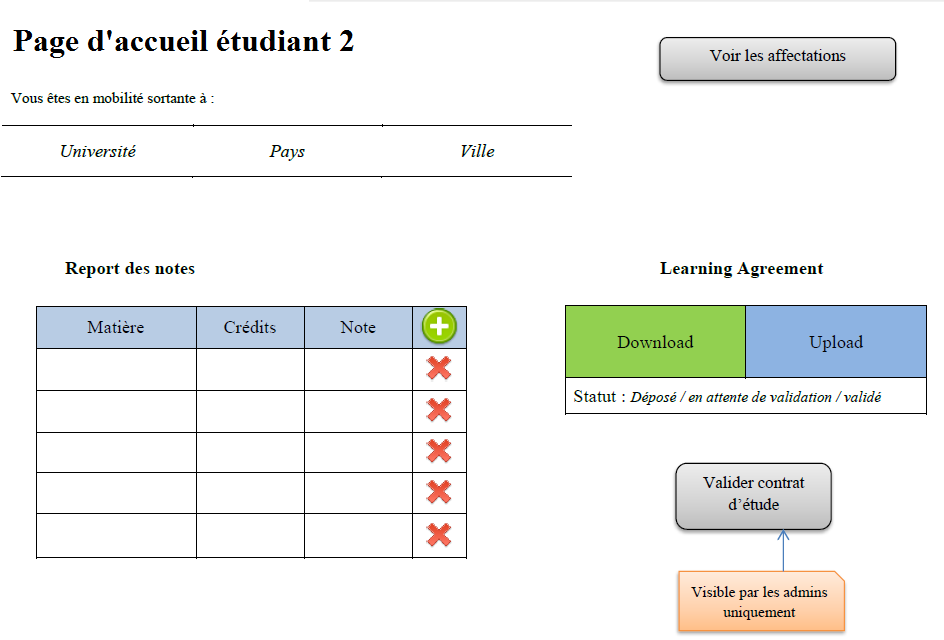
\includegraphics[scale=0.6]{Etudiant/HPS2.PNG}
	\caption{Page d'accueil pour les étudiants dans l'étape 2}
\end{figure}


Cette page est la nouvelle page d'accueil du site une fois l'étape 1 validée.
Elle est comme précédemment propre à chaque étudiant suivant sa destination. De nouvelles informations sont présentes ici.
On peut donc voir ici la destination assignée à l'étudiant en question, avec un lien vers sa "Fiche Université"(cf section \ref{sec::sheet_univ}).

L'élève peut accéder aux vœux des autres étudiants via un bouton "Vœux des Étudiants" (cf section \ref{sec::stud_wish}).
C'est sur cette page qu'est présente la gestion du téléchargement et du dépôt du Learning Agreement, avec un bouton pour télécharger un exemplaire vierge et un bouton pour déposer le document rempli.

Celui-ci est ensuite en attente de validation par le correspondant RI. On peut suivre ici les étapes de validation du Learning Agreement (à déposer, en attente de validation, validé).


\bigbreak

On pourra également trouver un tableau des matières choisies par l'élève qui seront validées par le correspondant RI dans le Learning Agreement.

\subsection{Admin}

L'administrateur (le correspondant RI) peut accéder à cette page avec des fonctionnalités supplémentaires.
Il peut supprimer ou valider/fixer les vœux de l'étudiant manuellement sur cette page (l'étudiant n'interviendra pas dans l'algorithme de sélection).

Le correspondant RI peut valider ici le Learning Agreement et les matières pour un étudiant en particulier.
